%!TEX root = lec05_query_processing.tex

%
% --------------------------------------------------------
%
\begin{frame}{Cost model for query processing}

Because I/O operations are much more costly than CPU operations, we are not concerned with algorithmic cost (as in CMPUT204).

\vskip0.5em

Instead, we \alert{measure the cost of a query} plan by:\\
 (1) \underline{the number of I/O operations} and \\
 (2) \underline{the number of memory buffers} needed to execute it.\footnote{The more memory a plan requires the more likely it is to incur costly I/O operations due to swapping.}

\vskip0.5em

\begin{BOX}{Assumptions}
- Each memory buffer holds \textbf{one} disk block

- Each I/O operation reads/writes a single block/buffer at a time

- The size of a database file is measured in blocks
\end{BOX}
\vskip0.5em

\end{frame}


%
% ------------------------------------------------
%
\begin{frame}{Table scans}

The \textbf{table scan} is the simplest way to get tuples from a table. It goes over every tuple in every block (recall slide~\ref{table_scan_iterator}).

\vskip1em

\begin{center}
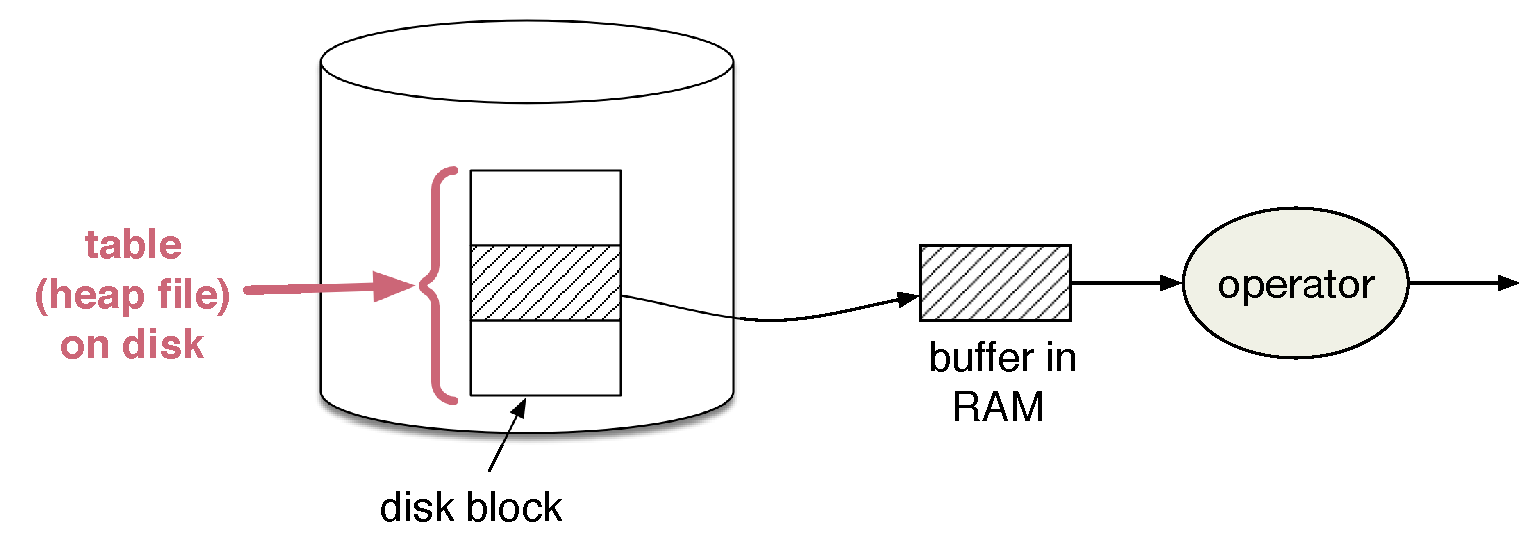
\includegraphics[width=0.75\textwidth]{figures/simple_table_scan}
\end{center}

A table scan requires only one buffer of RAM (which can be reused). But its I/O cost is $O(|R|)$ (as it goes over every disk block).

\end{frame}

%
% ------------------------------------------------
%
\begin{frame}{How do we find the cost of a plan?}

Focus on the iterators that perform I/O or store data in memory.

\vskip2em

\begin{columns}[onlytextwidth]
\begin{column}{0.125\textwidth}
	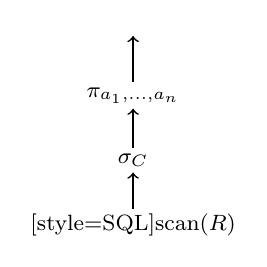
\begin{tikzpicture}[semithick,align=center,node distance=0.825cm,every node/.style={inner sep=1,outer sep=1,font=\footnotesize}]
	\node (0) at (0,0) {};
	\node (1) [below of=0] {$\pi_{a_1,\ldots,a_n}$};
    \node (2) [below of=1] {$\sigma_C$};
	\node (3) [below of=2] {\lstinline[style=SQL]{scan}($R$)};
    \path[->]
    	(1) edge (0)
        (2) edge (1)
        (3) edge (2);
	\end{tikzpicture}
\end{column}
\begin{column}{0.75\textwidth}
Recall that the iterators for $\sigma$ and $\pi$ do not read any data from disk, thus have 0 I/O cost. \\[1em]

Also, they do not need to keep any data in buffers. So their memory cost is also 0.
\end{column}
\end{columns}

\vskip2em

So the final cost of the plan is
\begin{center}
 \fbox{\alert{$O(1)$ buffers} in RAM} and \fbox{\alert{$O(|R|)$ I/O} operations}
\end{center} 
\end{frame}

%
% ------------------------------------------------
%
\begin{frame}{How many buffers should the DBMS use?}

\vskip1em

A complete table scan \underline{can be done with a single buffer}.

\vskip1em

But... IF there is more RAM available, \alert{should the DBMS read more blocks at once (maybe all of them) OR ... should it save RAM}?

\vskip1em

Reading many consecutive blocks at once is better:\\
 - this amortizes the seek time (for HDDs) and\\
 - reduces the impact of BUS congestion

\end{frame}


%
% ------------------------------------------------
%

\floatstyle{plaintop}
\restylefloat{algorithm}

\newsavebox\nestedLoopJoinAlgorithm
\savebox{\nestedLoopJoinAlgorithm}{
\begin{minipage}{0.7\textwidth}%
\begin{algorithm}[H]
\begin{algorithmic}
% \caption{evaluating $R \Join_C S$}
\ForEach {buffer $b_R$ of $R$}
	\ForEach {buffer $b_S$ of $S$}
		\ForEach {tuple $t_R$ in $b_R$}
			\ForEach {tuple $t_S$ in $b_S$}
				\State $t' \leftarrow \text{join}(t_R,t_S)$ 
				\If {$t'$ satisfies $C$}
					\State \Return $t'$ 
				\EndIf
			\EndFor
		\EndFor
	\EndFor
\EndFor
\end{algorithmic}
\end{algorithm}
\end{minipage}}

\begin{frame}{The I/O cost of joins and products}
\label{nested_loop_join}

To find out \textbf{the actual I/O cost} of the nested-loop-join algorithm of slide~\ref{nested_loop_join_iterator}, consider what happens when we take the calls to \lstinline[style=SQL]{GetNext()} in table scans into account:

\vspace*{-1em}

\begin{columns}
\begin{column}{0.5\textwidth}
\begin{center}
\scalebox{0.75}{\usebox\nestedLoopJoinAlgorithm}
\label{alg:nested_loop_join}
\end{center}
\end{column}

\begin{column}{0.3\textwidth}
\begin{center}
	\begin{tikzpicture}[semithick,align=center,node distance=0.825cm,every node/.style={inner sep=1,outer sep=1,font=\footnotesize}]
	\node (0) at (0,0) {};
    \node (1) [below of=0] {$\Join_C$};
	\node (2) [below of=1,xshift=-1cm] {\lstinline[style=SQL]{scan}($R$)};
	\node (3) [below of=1,xshift=1cm] {\lstinline[style=SQL]{scan}($S$)};

    \path[commutative diagrams/.cd, every arrow, every label]
        (1) edge (0)
        (2) edge (1)
        (3) edge (1);
	\end{tikzpicture}
\end{center}
\end{column}
\end{columns}

So, how many block reads are done?

\end{frame}

%
% ------------------------------------------------
%
\begin{frame}

\vskip1em

\begin{columns}[onlytextwidth]
\begin{column}{0.6\textwidth}
\textbf{Case 1:} use \underline{one} buffer for each scan.
\\[1em]
Memory Cost = 2 buffers\\
I/O Cost = \onslide<2->{\fbox{$O(|R| \cdot |S|)$ block reads}}
\end{column}
\begin{column}{0.45\textwidth}
\scalebox{0.55}{\usebox\nestedLoopJoinAlgorithm}
\end{column}
\end{columns}

\vskip1em

\onslide<2-> \alert{This is the worst case scenario for I/O: quadratic number of block reads.}


\end{frame}


\begin{frame}

\vskip1em

\begin{columns}[onlytextwidth]
\begin{column}{0.6\textwidth}
\textbf{Case 2:} we have $M$ buffers available and $|S| < M-1$.
\end{column}
\begin{column}{0.45\textwidth}
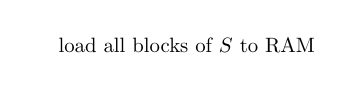
\begin{tikzpicture}
\node at (0,0) [anchor=north west] {\scalebox{0.75}{\alert{load all blocks of $S$ to RAM}}};
\node at (-0.275,0.0125) [anchor=north west]{\scalebox{0.65}{\usebox\nestedLoopJoinAlgorithm}};
\end{tikzpicture}

\end{column}
\end{columns}

\vskip1em

The best case here is to use \underline{one} buffer to scan for $R$, and to \textbf{load all blocks of $S$} to buffers in RAM \alert{beforehand}.

Note that no tuple of either table is read from disk more than once.

\vskip0.5em

\begin{center}
Memory Cost = \onslide<2->{\fbox{$|S|+1$}} and I/O Cost = \onslide<3->{\fbox{$|R|+|S|$}}
\end{center}
\end{frame}

%
% ------------------------------------------------
%
\begin{frame}


\textbf{Case 3:}  $M$ buffers available and $M<|S|\leq|R|$.

Now the best way is to break the inner table into \emph{chunks} of $M-1$ blocks, and make multiple passes on $R$ using a single buffer:

\begin{tikzpicture}
\node at (0,0) {\scalebox{0.75}{\begin{minipage}{1.2\textwidth}%
\begin{algorithm}[H]
\begin{algorithmic}
\ForEach {\alert{chunk of $M-1$ blocks of $S$}}
\ForEach {buffer $b_R$ of $R$}
	\ForEach {tuple $t_R$ in $b_R$}
		\ForEach {buffer $b_S$ of $S$ \alert{in memory}}
			\ForEach {tuple $t_S$ in $b_S$}
				\State $t' \leftarrow \text{\alert{join}}(t_R,t_S)$ 
				\If {$t'$ satisfies $C$}
					\State return $t'$ 
				\EndIf
			\EndFor
		\EndFor
	\EndFor
\EndFor
\EndFor
\end{algorithmic}
\end{algorithm}
\end{minipage}}};

\node at (4.5,-0.25) {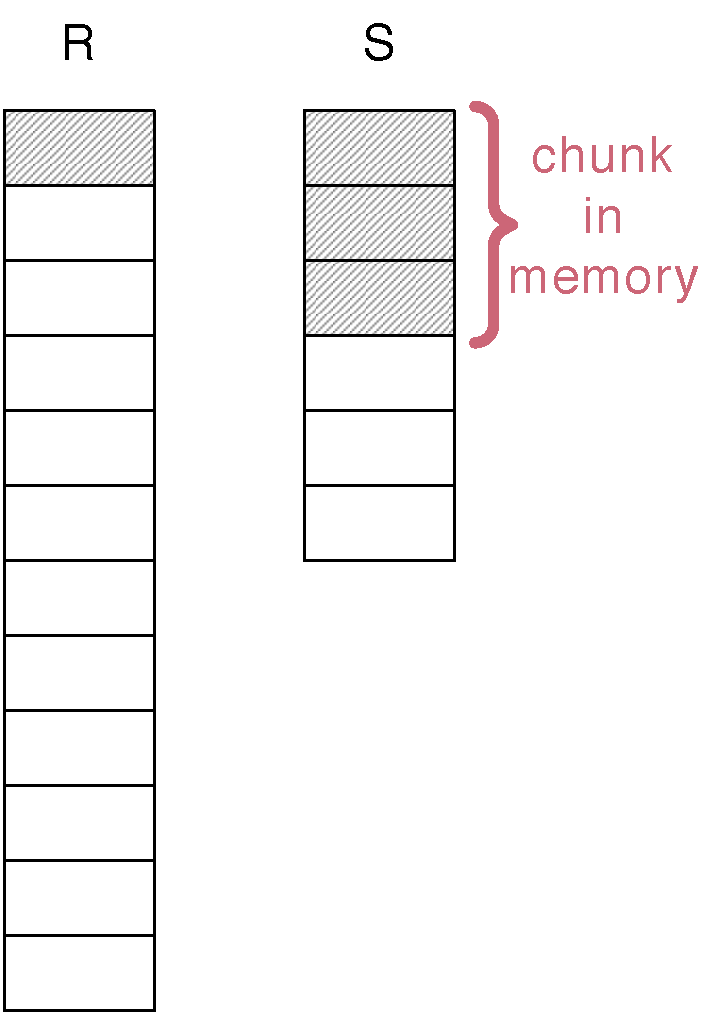
\includegraphics[width=0.3\textwidth]{figures/nested_loop_join.pdf}};

\end{tikzpicture}
\end{frame}

%
% ------------------------------------------------
%
\begin{frame}
\label{example_cost_nested_loop_join}
Cost:

\vskip2em

\begin{columns}[onlytextwidth]
\begin{column}{0.6\textwidth}

I/O: \(\ceil*{\frac{|S|}{M-1}}(|R|) + |S|\) block reads

\vskip1em

Memory: $M$ buffers

\vskip2em

\textbf{Example}:\\
- $|R|$ = 12 disk blocks\\
- $|S|$ = 6 disk blocks\\
- $M=4$ memory buffers available

\vskip2em

$\ceil*{\frac{6}{3}} = 2$ chunks;\\ total cost = $(2\cdot 12)+6 = 30$ block reads.
\end{column}
\begin{column}{0.4\textwidth}
\flushright 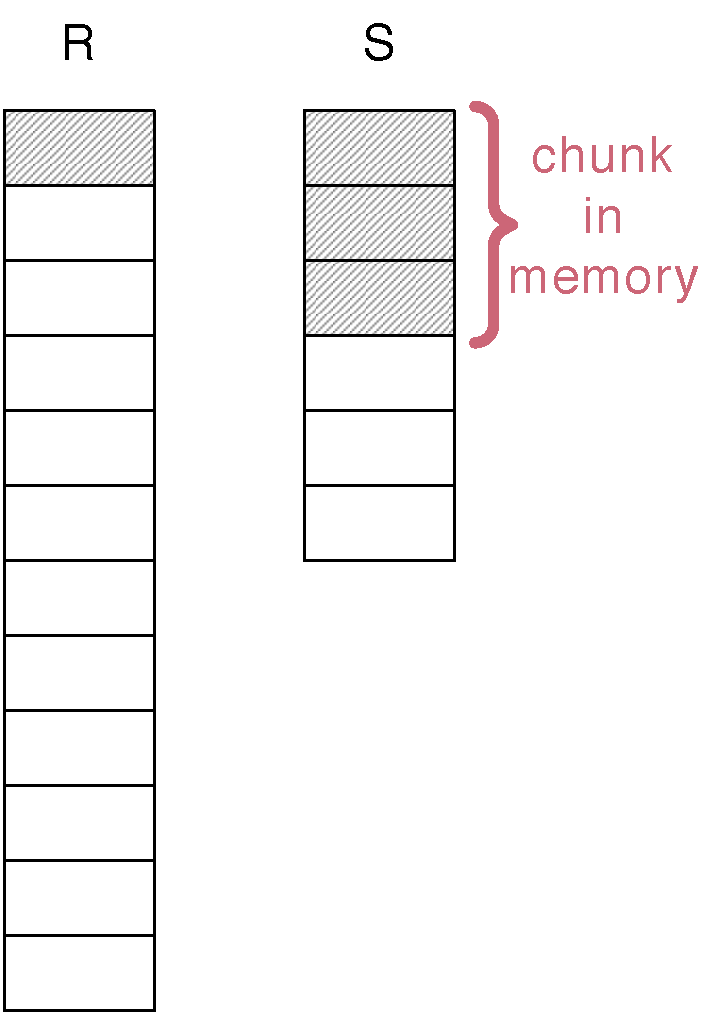
\includegraphics[width=0.75\textwidth]{figures/nested_loop_join.pdf}
\end{column}
\end{columns}
\end{frame}

%
% ------------------------------------------------
%
\begin{frame}{Speeding up the nested loop join}
\label{nested_loop_join_with_indexing_inner_table}

To find matching pairs of tuples faster, the DBMS may \alert{\underline{sort} the tuples of S in memory} (by the join attributes).

If the join is based on an equality (\lstinline[style=SQL]{S.a = R.b}), the DBMS may \alert{build a \underline{hash} table with the tuples of S} (key: \lstinline[style=SQL]{S.a}, value: whole tuple).

\begin{center}
\begin{tikzpicture}[semithick,every node/.style={inner sep=1,outer sep=1,font=\footnotesize}]
\node at (0,0) {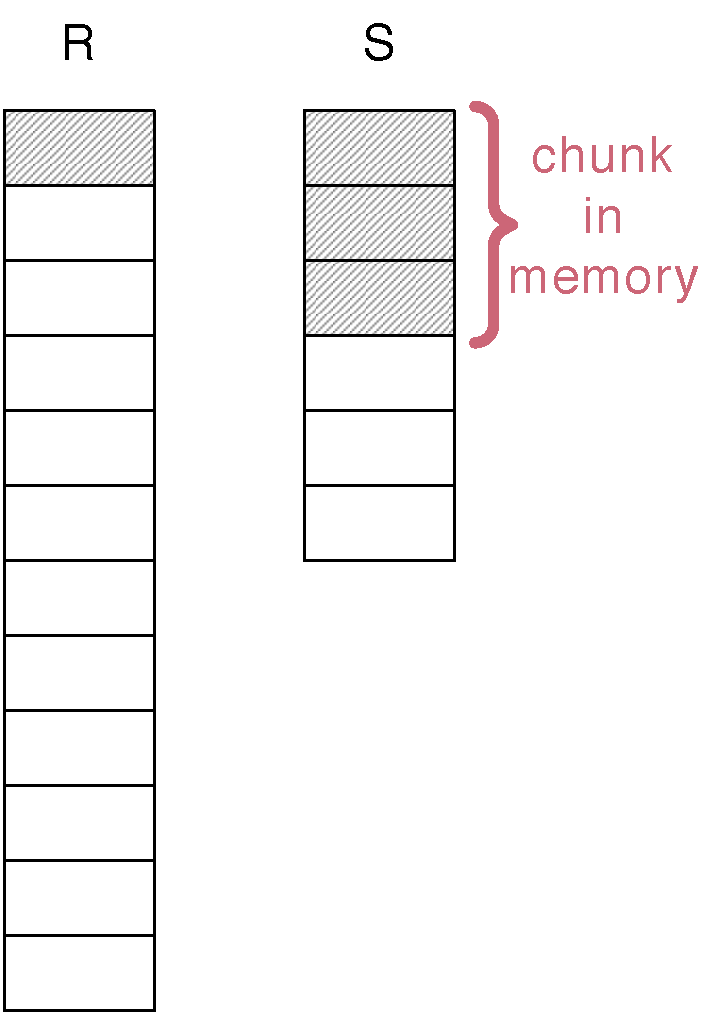
\includegraphics[width=0.3\textwidth]{figures/nested_loop_join.pdf}};

\node (0) at (4,1) [draw,color=accent] {\begin{minipage}{2.15cm}\baselineskip=0.75\baselineskip \centering
sorted/hashed by the join attributes!\end{minipage}};

\draw [->,color=accent] (0) -- (1.75,1.25);
\end{tikzpicture}
\end{center}
\end{frame}

\begin{frame}[fragile]

Example: sorting the results of a sub-expression.

\vskip1em

\begin{columns}[onlytextwidth]
\begin{column}{0.5\textwidth}
\begin{lstlisting}[style=SQL]
SELECT role, imdb
FROM Movie JOIN Cast
WHERE actor='Bill Murray'
\end{lstlisting}
\end{column}
\begin{column}{0.6\textwidth}
\begin{tikzpicture}[semithick,align=center,node distance=0.875cm,every node/.style={inner sep=1,outer sep=1,font=\footnotesize}]
\node (0) at (0,0) {} ; %empty node with ``answer''
\node (1) [below of= 0] {$\pi_{\texttt{role,imdb}}$};
\node (2) [below of= 1] {$\Join$};
\node (3a) [below right of= 2, xshift=1cm] {\lstinline[style=SQL]{sort_by(title,year)}};
\node (3) [below of= 3a] {$\sigma_{\texttt{actor='Bill Murray'}}$};
\node (4) [below left of= 2, xshift=-1cm] {\lstinline[style=SQL]{scan(Movie)}};
\node (5) [below of = 3] {\lstinline[style=SQL]{scan(Cast)}};
\path[->]
    (4) edge (2)
    (5) edge (3) 
    (3) edge (3a)
    (3a) edge (2)
    (2) edge (1)
    (1) edge (0);
\end{tikzpicture}

\end{column}
\end{columns}

\vskip1em

Better yet, we could sort the results of \textbf{both} sub-expressions on the join attributes and perform a sort-based-join (see slide~\ref{sort_based_equality_join_idea}) in memory.

\end{frame}


% \begin{frame}
% \begin{tikzpicture}[semithick,align=center,node distance=0.875cm,every node/.style={inner sep=1,outer sep=1,font=\footnotesize}]
% \node (0) at (0,0) {} ; %empty node with ``answer''
% \node (1) [below of= 0] {$\pi_{\texttt{a,e}}$};
% \node (2) [below of= 1] {$\Join$};
% \node (3) [below right of= 2, xshift=1cm] {\lstinline[style=SQL]{sort_by(a,b)}};
% \node (4) [below left of= 2, xshift=-1cm] {\lstinline[style=SQL]{scan(S)}};
% \node (5) [below of = 3] {\lstinline[style=SQL]{scan(R)}};
% \path[->]
%     (4) edge (2)
%     (5) edge (3) 
%     (3) edge (2)
%     (2) edge (1)
%     (1) edge (0);
% \end{tikzpicture}

% \end{frame}


%
% ------------------------------------------------
%
\begin{frame}{Computing set operations with sorting/hashing}
\label{set_union_one_pass}
\begin{columns}[onlytextwidth]
\begin{column}{0.6\textwidth}

\alert{Set Union $R\cup S$}:

\vskip0.5em

Assumptions:\\
 - $M$ buffers available\\ 
 - $|R| > |S|$ and $|R \cup S| \leq M-1$
\end{column}
\begin{column}{0.4\textwidth}
\flushright\usebox{\genericSetOperator}
\end{column}
\end{columns}

\vskip2em

\begin{enumerate}[label=(\arabic*)]
\item Keep a hash set $H_S$ in memory.

\item Read each block of $S$ using a single buffer $b_S$;
\begin{itemize}[-,topsep=-0.5em]
\item For each $t_S$ in $b_S$: if it is not in $H_S$, add it to $H_S$ and return it to the caller.
\end{itemize}


\item Read each block of $R$ using a single buffer $b_R$;
\begin{itemize}[-,topsep=-0.5em]
\item For each $t$ in $b_R$: if it is not in $H_S$, add it to $H_S$ and return it to the caller.
\end{itemize}

\end{enumerate}
\end{frame}




%
% ------------------------------------------------
%
\begin{frame}
\label{set_intersection_one_pass}
\begin{columns}[onlytextwidth]
\begin{column}{0.6\textwidth}

\alert{Set Intersection $R\cap S$}:

\vskip0.5em

Assumptions:\\
 - $M$ buffers available\\ 
 - $|R| > |S|$ and $|S| \leq M-1$
\end{column}
\begin{column}{0.4\textwidth}
\flushright\usebox{\genericSetOperator}
\end{column}
\end{columns}

\vskip2em

\begin{enumerate}[label=(\arabic*)]
\item Read \underline{all of $S$} into a hash set (size $M-1$ buffers) in memory.

\item Read each block of $R$ to (single) buffer $b_R$;
\begin{itemize}[-,topsep=-0.5em]
\item For each $t$ in $b_R$: if it is in $H_S$, \alert{remove it from $H_S$} and return it to the caller.
\end{itemize}
\end{enumerate}
\end{frame}


%
% ------------------------------------------------
%
\begin{frame}
\label{set_difference_left_one_pass}
\begin{columns}[onlytextwidth]
\begin{column}{0.6\textwidth}

\alert{Set Difference $R - S$ (Algorithm 1)}:

\vskip0.5em

Assumptions:\\
 - $M$ buffers available\\ 
 - \blue{$|R| > |S|$} and $|S \cup (R-S)| \leq M-1$
\end{column}
\begin{column}{0.4\textwidth}
\flushright\usebox{\genericSetOperator}
\end{column}
\end{columns}

\vskip2em

\begin{enumerate}[label=(\arabic*)]
\item Read all of $S$ into a hash set $H_S$ in memory.

\item Read each block of $R$ to (single) buffer $b_R$;
\begin{itemize}[-,topsep=-0.5em]
\item For each $t$ in $b_R$: if it is not in $H_S$, \underline{add it to $H_S$} and return it to the caller.
\end{itemize}
\end{enumerate}
\end{frame}


%
% ------------------------------------------------
%
\begin{frame}
\label{set_difference_right_one_pass}
\begin{columns}[onlytextwidth]
\begin{column}{0.6\textwidth}

\alert{Set Difference $R - S$ (Algorithm 2)}

\vskip0.5em

Assumptions:\\
 - $M$ buffers available\\ 
 - \blue{$|S| > |R|$} and $|R| \leq M-1$
\end{column}
\begin{column}{0.4\textwidth}
\flushright\usebox{\genericSetOperator}
\end{column}
\end{columns}

\vskip2em

\begin{enumerate}[label=(\arabic*)]
\item Read all of $R$ into a hash set $H_R$ in memory.

\item Read each block of $S$ to (single) buffer $b_S$;
\begin{itemize}[-,topsep=-0.5em]
\item For each $t_S$ in $b_S$: if \alert{$t_S$ \textbf{is} in $H_R$} remove it from $H_R$.
\end{itemize}

\item Return the tuples in $H_R$ (one at a time) to the caller.
\end{enumerate}
\end{frame}


%
% ------------------------------------------------
%

\newsavebox{\DISTINCTQUERY}
\begin{lrbox}{\DISTINCTQUERY}
\begin{minipage}{0.5\textwidth}
\begin{lstlisting}[style=SQL,escapeinside={(*}{*)},frame=single]
SELECT DISTINCT (*$a_1$*), ... , (*$a_n$*)
FROM (*$T_1$*) [, (*$T_2$*) [, (*$\ldots$*) [, (*$T_m$*)]]]
WHERE (*$c_1$*) AND (*$c_2$*) AND (*\ldots*) AND (*$c_k$*)
\end{lstlisting}
\end{minipage}
\end{lrbox}

\begin{frame}[fragile]{Duplicate elimination}
\label{duplicate_elimination}

\begin{columns}[onlytextwidth]
\begin{column}{0.7\textwidth}

Removing duplicates is done last in the plan!

\vskip1em

\textbf{Idea}: keep the tuples from the query (\alert{$Q$}) in a hash set, using \underline{up to} $M$ buffers; discard duplicates as they arrive (see slide~\ref{distinct_iterator}).

\vskip1em

\begin{center}
\scalebox{0.75}{\usebox{\DISTINCTQUERY}}
\end{center}


\vskip1em

Assumption: $|\alert{Q}| < M$
\vskip0.5em

Cost = \fbox{0 I/O} and \fbox{$O(|\alert{Q}|)$ buffers.}

\end{column}

\begin{column}{0.3\textwidth}
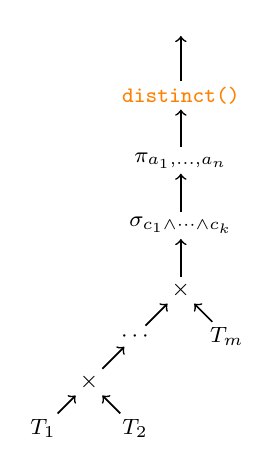
\begin{tikzpicture}[semithick,align=center,node distance=0.825cm,every node/.style={inner sep=1,outer sep=1,font=\footnotesize}]
	\node (0) at (0,0) {};
    \node (1) [below of=0] {\textcolor{orange}{\texttt{distinct()}}};
	\node (2) [below of=1] {$\pi_{a_1,\ldots,a_n}$};
	\node (3) [below of=2] {$\sigma_{c_1 \wedge \cdots \wedge c_k}$};
	\node (4) [below of=3] {$\times$};
	\node (5) [below left of=4] {$\cdots$};
	\node (6) [below right of=4] {$T_m$};
	\node (7) [below left of=5] {$\times$};
	\node (8) [below left of=7] {$T_1$};
	\node (9) [below right of=7] {$T_2$};
    \path[->]
        (1) edge (0)
        (2) edge (1)
        (3) edge (2)
        (4) edge (3)
        (5) edge (4)
        (6) edge (4)
        (7) edge (5)
        (8) edge (7)
        (9) edge (7);
\end{tikzpicture}
\end{column}
\end{columns}
\end{frame}



